
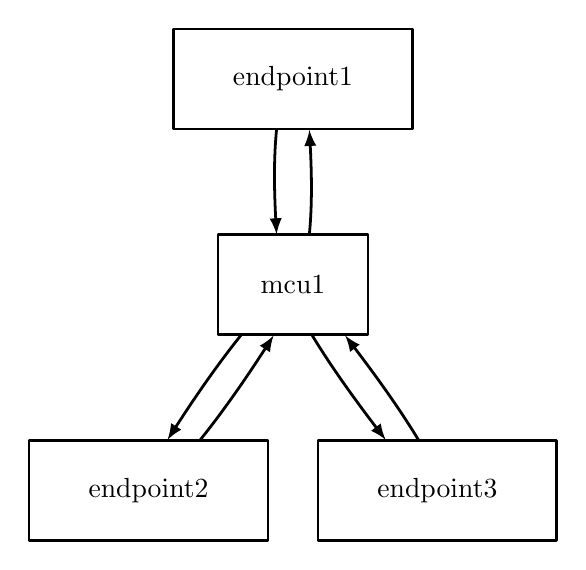
\begin{tikzpicture}[>=latex,line join=bevel,]
  \pgfsetlinewidth{1bp}
%%
\pgfsetcolor{black}
  % Edge: mcu1 -> endpoint3
  \draw [->] (101.94bp,74.708bp) .. controls (107.36bp,65.747bp) and (114.87bp,54.799bp)  .. (128.4bp,37.082bp);
  % Edge: mcu1 -> endpoint2
  \draw [->] (76.23bp,74.708bp) .. controls (69.202bp,65.926bp) and (61.494bp,55.236bp)  .. (49.811bp,37.082bp);
  % Edge: endpoint1 -> mcu1
  \draw [->] (89.084bp,148.71bp) .. controls (88.271bp,140.37bp) and (88.052bp,130.32bp)  .. (89.105bp,111.08bp);
  % Edge: endpoint2 -> mcu1
  \draw [->] (61.601bp,37.082bp) .. controls (68.618bp,45.833bp) and (76.332bp,56.516bp)  .. (88.062bp,74.708bp);
  % Edge: endpoint3 -> mcu1
  \draw [->] (140.19bp,37.082bp) .. controls (134.8bp,46.012bp) and (127.31bp,56.953bp)  .. (113.77bp,74.708bp);
  % Edge: mcu1 -> endpoint1
  \draw [->] (100.9bp,111.08bp) .. controls (101.72bp,119.39bp) and (101.95bp,129.43bp)  .. (100.92bp,148.71bp);
  % Node: endpoint1
\begin{scope}
  \definecolor{strokecol}{rgb}{0.0,0.0,0.0};
  \pgfsetstrokecolor{strokecol}
  \draw (52bp,149bp) -- (52bp,185bp) -- (138bp,185bp) -- (138bp,149bp) -- cycle;
  \draw (95bp,167bp) node {endpoint1};
\end{scope}
  % Node: endpoint2
\begin{scope}
  \definecolor{strokecol}{rgb}{0.0,0.0,0.0};
  \pgfsetstrokecolor{strokecol}
  \draw (0bp,1bp) -- (0bp,37bp) -- (86bp,37bp) -- (86bp,1bp) -- cycle;
  \draw (43bp,19bp) node {endpoint2};
\end{scope}
  % Node: endpoint3
\begin{scope}
  \definecolor{strokecol}{rgb}{0.0,0.0,0.0};
  \pgfsetstrokecolor{strokecol}
  \draw (104bp,1bp) -- (104bp,37bp) -- (190bp,37bp) -- (190bp,1bp) -- cycle;
  \draw (147bp,19bp) node {endpoint3};
\end{scope}
  % Node: mcu1
\begin{scope}
  \definecolor{strokecol}{rgb}{0.0,0.0,0.0};
  \pgfsetstrokecolor{strokecol}
  \draw (68bp,75bp) -- (68bp,111bp) -- (122bp,111bp) -- (122bp,75bp) -- cycle;
  \draw (95bp,93bp) node {mcu1};
\end{scope}
%
\end{tikzpicture}

